% Propósito: ordenar las etapas de la audición periférica y distinguir los
% dominios físico, celular y neural sin sugerir creación de energía.
% Origen: cadena funcional descrita en la sección
% \ref{sec:u6-cadena}. No representa escalas anatómicas ni una medición.
% Descripción accesible: siete bloques conectados siguen la transformación
% desde la presión acústica en el aire hasta la actividad del nervio auditivo.
% Los bloques cambian de sombreado al pasar por las etapas acústica, mecánica,
% hidromecánica, celular y neural. Una nota inferior aclara que el sistema
% transforma y disipa energía, mientras las células ciliadas externas aportan
% un proceso activo alimentado por el metabolismo.
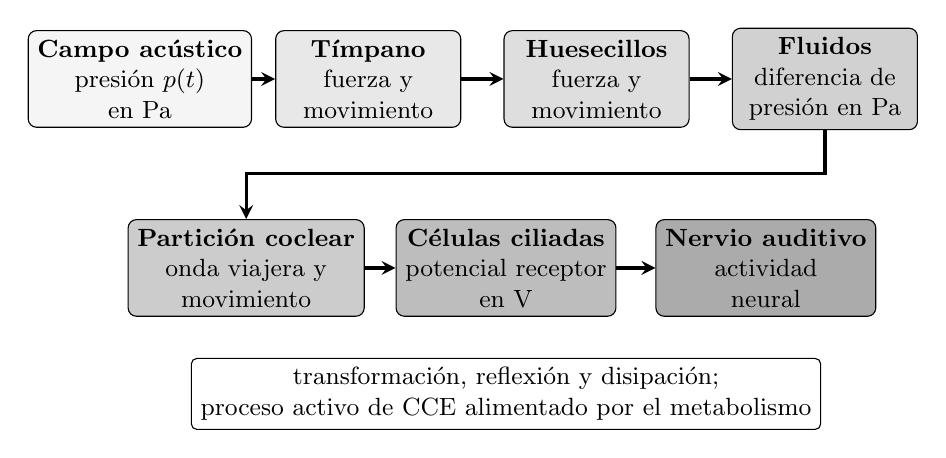
\begin{tikzpicture}[font=\small,>=stealth,x=1cm,y=1cm]
    \tikzset{
        stage/.style={
            draw,
            rounded corners=3pt,
            minimum width=2.35cm,
            minimum height=1.10cm,
            align=center
        },
        link/.style={->,very thick}
    }

    \node[stage,fill=black!4] (air) at (1.35,3.35)
        {\textbf{Campo acústico}\\presión \(p(t)\)\\en Pa};
    \node[stage,fill=black!9] (tm) at (4.25,3.35)
        {\textbf{Tímpano}\\fuerza y\\movimiento};
    \node[stage,fill=black!13] (oss) at (7.15,3.35)
        {\textbf{Huesecillos}\\fuerza y\\movimiento};
    \node[stage,fill=black!18] (fluid) at (10.05,3.35)
        {\textbf{Fluidos}\\diferencia de\\presión en Pa};

    \node[stage,fill=black!20] (partition) at (2.70,0.95)
        {\textbf{Partición coclear}\\onda viajera y\\movimiento};
    \node[stage,fill=black!26] (hair) at (6.00,0.95)
        {\textbf{Células ciliadas}\\potencial receptor\\en V};
    \node[stage,fill=black!33] (nerve) at (9.30,0.95)
        {\textbf{Nervio auditivo}\\actividad\\neural};

    \draw[link] (air.east) -- (tm.west);
    \draw[link] (tm.east) -- (oss.west);
    \draw[link] (oss.east) -- (fluid.west);
    \draw[link] (fluid.south) -- ++(0,-0.55) -| (partition.north);
    \draw[link] (partition.east) -- (hair.west);
    \draw[link] (hair.east) -- (nerve.west);

    \node[align=center,draw,rounded corners=2pt,fill=white] at (6.00,-0.65)
        {transformación, reflexión y disipación;\\
         proceso activo de CCE alimentado por el metabolismo};
\end{tikzpicture}
